\documentclass[a4paper,12pt]{article}
\usepackage[utf8]{inputenc}
\usepackage[brazil]{babel}
\usepackage{multirow}
\usepackage{booktabs}
\usepackage{enumitem}
\usepackage{setspace}
\setstretch{1.5}
\usepackage[lmargin=3cm,tmargin=3cm,rmargin=2cm,bmargin=2cm]{geometry} %Formato que lembra a ABNT
\usepackage[T1]{fontenc} %Ajusta o texto que vem de outras fontes
\usepackage{graphicx,xcolor,enumerate}




\begin{document}
\section{METODOLOGIA}
\hspace{0.5cm}A metodologia do projeto foi feita em três momentos. Primeiramente, com o levanta-
mento dos requisitos do software, que definiu os serviços que o software oferecerá. Em seguida,
é abordada quais ferramentas foram e quais serão utilizadas no desenvolvimento da aplicação.
Por fim, é apresentada a aplicação, com suas caraterísticas e fluxo de telas.
\subsection{LEVANTAMENTO DE REQUISITOS}
\hspace{0.5cm}O levantamento de requisitos para o desenvolvimento do projeto, foi feito através de dois
itens: diagrama de classes e casos de uso.
\clearpage
\subsubsection{Diagrama de classes}
\hspace{0.5cm}Nesse tópico, foi aplicado o diagrama de classes, para exibir as classes presentes no
sistema e seus respectivos atributos e métodos.
\begin{figure}[ht!]
    \centering
    \caption{Figura 1: Diagrama de Classe}
    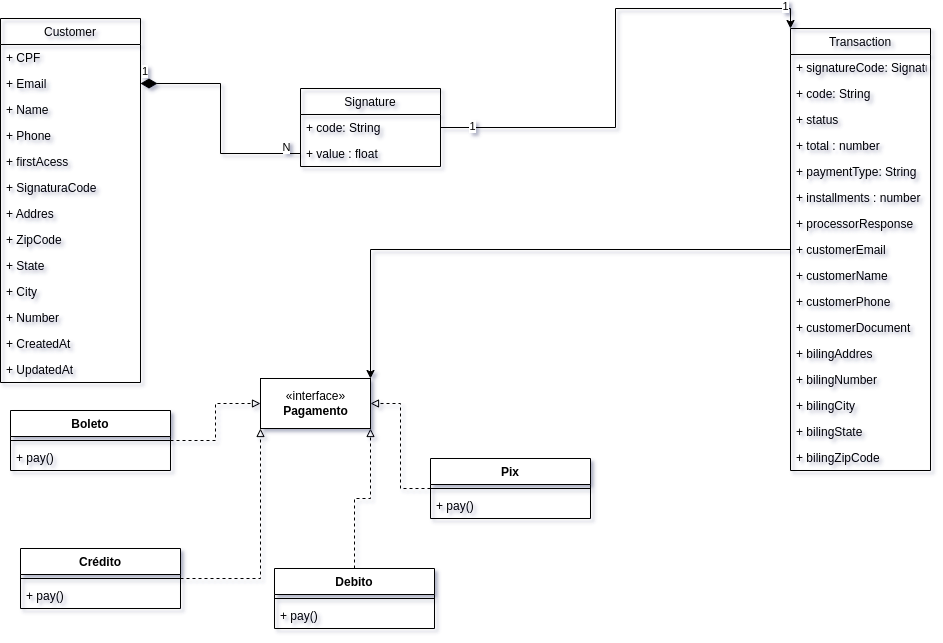
\includegraphics[width=15cm]{imagens/diagrama de Classe.png}
    \textbf{Fonte:} Elaborada pelo Autor
\end{figure}
\hspace{0.5cm}Primeiramente,o usuário pode assumir o papel de Admin ou Cliente,nunca os dois ao mesmo tempo, que define desempenham funções diferentes no sistema.
Adiante, as assinaturas faz o papel de gestor entre as transações e o cliente, logo um cliente pode ter apenas uma assinatura e assinatura pode pertencer a diferentes clientes,
Ademais, as transações recebem uma assinatura e dados de um cliente para serem realizadas e dependendo da interface de pagamento recebe essa transações seus atributos podem ser alterados
Por fim, a interface de pagamento depende do tipo de pagamento que o cliente deseja fazer, assim se adaptando a diferentes contextos de pagamentos

\newpage
\subsubsection{Casos de uso}
\hspace{0.5cm}Nesse item, foram utilizados os casos de uso, uma forma existente para especificar
as funcionalidades do software. Nas tabelas abaixo, foram abordadas sobre cada função o
ator principal, a descrição, o propósito, a pré-condição, o fluxo principal, e, se existir, o fluxo
alternativo e o fluxo exceção.
%Use Case 01
\begin{table}[ht]
    \centering
    \begin{tabular}{|p{3.5cm}|p{10cm}|p{7cm}|}
        \hline
        \textbf{UC-01}                  & \textbf{EFETUAR LOGIN}                                                           \\
        \hline

        \multirow{1}{*}{Ator principal} & Usuário                                                                          \\
        \hline
        \multirow{1}{*}{Descrição}      & Autenticação do usuário cadastrado no sistema, permitindo a realização
        de operações na área restrita do site.                                                                             \\
        \hline

        \multirow{1}{*}{Propósito}      & Acessar o sistema para ver pagamentos, sua assinatura..                          \\
        \hline

        \multirow{1}{*}{Pré-condição}   & O usuário deve estar cadastrado no sistema..                                     \\
        \hline

        \multirow{1}{*}{Fluxo principal}
                                        & Entrar pelo login;                                                               \\
                                        & O sistema solicita informações obrigatórias para a autenticação: e-mail e senha; \\
                                        & O usuário informa os dados de autenticação;                                      \\
                                        & O sistema habilita as ações relacionadas ao software.                            \\
        \cline{2-2}
        \hline

        \multirow{2}{*}{Fluxo Alternativo}
                                        & Opção voltar                                                                     \\
                                        & • O usuário seleciona a opção voltar;                                            \\
                                        & • O sistema retorna a tela anterior.                                             \\
                                        & • O usuário seleciona a opção esqueci a senha;                                   \\
                                        & • O sistema mostra uma tela para atualizar a senha;                              \\
                                        & • O usuário informa a nova senha;                                                \\
                                        & • A senha é atualizada;                                                          \\
                                        & • O sistema retorna a página de login.                                           \\
        \hline
        \multirow{2}{*}{Fluxo de Exceção}
                                        & Informações obrigatórias para a autenticação incorretas:                         \\
                                        & • O sistema informa ao usuário o erro.                                           \\
        \hline
    \end{tabular}
    \caption{Tabela de Caso de Uso de Realizar Login}
    \label{tab:casos-de-uso}
\end{table}

%UseCase 02
\begin{table}[ht]
    \centering
    \begin{tabular}{|p{3.5cm}|p{10cm}|p{7cm}|}
        \hline
        \textbf{UC-02}                     & \textbf{Realizar cadastro}                                                               \\
        \hline

        \multirow{1}{*}{Ator principal}    & Admin                                                                                    \\
        \hline
        \multirow{1}{*}{Descrição}         & Cadastro do cliente, que vai permitir o login e acesso ao software.                      \\
        \hline

        \multirow{1}{*}{Propósito}         & Acessar o sistema para ver pagamentos, sua assinatura..                                  \\
        \hline

        \multirow{1}{*}{Pré-condição}      & O Cliente deve ter email unico, que não consta na base de dados e informações válidas    \\
                                           & Admin Deve conhecer uma senha especial para fornecer ao sistema                          \\
        \hline

        \multirow{1}{*}{Fluxo principal}
                                           & • Entrar pelo login;                                                                     \\
                                           & • O sistema retorna a página inicial e possuindo a opção de cadastrar novos clientes com \\
                                           & • O Admin informa os dados de cadastro;                                                  \\
                                           & • O sistema habilita as ações relacionadas ao software para o usuário.                   \\
        \cline{2-2}
        \hline

        \multirow{1}{*}{Fluxo Alternativo} & N/A                                                                                      \\
        \hline

        \multirow{2}{*}{Fluxo de Exceção}
                                           & Campos obrigatórios                                                                      \\
                                           & • O sistema verifica que os campos obrigatórios não forma preenchi-
        dos;                                                                                                                          \\
                                           & • O sistema exibe mensagem de alerta.                                                    \\
                                           & E-mail já existente                                                                      \\
                                           & • O sistema verifica que o e-mail informado já está cadastrado no
        sistema;                                                                                                                      \\
                                           & • O sistema exibe mensagem de alerta.                                                    \\
        \hline
    \end{tabular}
    \caption{Tabela de Caso de Uso de Realizar Cadastro}
\end{table}
%UseCase 03
\begin{table}[ht]
    \centering
    \begin{tabular}{|p{3.5cm}|p{10cm}|p{7cm}|}
        \hline
        \textbf{UC-03}                     & \textbf{Realizar cadastro de uma Assinatura}                                                                     \\
        \hline

        \multirow{1}{*}{Ator principal}    & Admin                                                                                                            \\
        \hline
        \multirow{1}{*}{Descrição}         & Cadastro das assinaturas, que permite indentificar o plano do usuário                                            \\
        \hline

        \multirow{1}{*}{Propósito}         & Permitir o usuário paga sua assinatura..                                                                         \\
        \hline

        \multirow{1}{*}{Pré-condição}      & O Admin deve está logado para criar as assinaturas                                                               \\
        \hline

        \multirow{1}{*}{Fluxo principal}
                                           & • Entrar pelo login;                                                                                             \\
                                           & • A Home Possui um botão que indica a criação de assinaturas                                                     \\
                                           & • O Admin informa os dados da assinatura;                                                                        \\
                                           & • O sistema habilita as ações relacionadas ao usuário poder tem aquela assinatura.                               \\
        \cline{2-2}
        \hline

        \multirow{1}{*}{Fluxo Alternativo} & N/A                                                                                                              \\
        \hline

        \multirow{2}{*}{Fluxo de Exceção}
                                           & Caso o Admin não esteja logado ou quem quer criar a assinatura não seja admin                                    \\
                                           & • O Sistema verifica a identidade do usuário e caso ele não seja admin não deixa continuar e exibi uma mensagem; \\
                                           & • O sistema exibe mensagem de alerta.                                                                            \\
        \hline
    \end{tabular}
    \caption{Tabela de Caso de Uso de Criar uma Assinatura}
\end{table}

%UseCase 04
\begin{table}[ht]
    \centering
    \begin{tabular}{|p{3.5cm}|p{10cm}|p{7cm}|}
        \hline
        \textbf{UC-04}                     & \textbf{Apagar nos registro  uma Assinatura}                                                                                                                              \\
        \hline

        \multirow{1}{*}{Ator principal}    & Admin                                                                                                                                                                     \\
        \hline
        \multirow{1}{*}{Descrição}         & Excluir dos registros uma assinatura que não faz mais parte do contexto do sistema                                                                                        \\
        \hline

        \multirow{1}{*}{Propósito}         & Manter Limpo os Registros que não vão mais ser ultilizados..                                                                                                              \\
        \hline

        \multirow{1}{*}{Pré-condição}      & O Admin deve está logado para apagar as assinaturas                                                                                                                       \\
        \hline

        \multirow{1}{*}{Fluxo principal}
                                           & • Entrar pelo login;                                                                                                                                                      \\
                                           & • A Home Possui um botão que leva para ver todas as assinaturas e caso o haja a necessidade de excluir a assinatura é apagada do sistemas sem prejudicar outras entidades \\
        \cline{2-2}
        \hline

        \multirow{1}{*}{Fluxo Alternativo} & N/A                                                                                                                                                                       \\
        \hline

        \multirow{2}{*}{Fluxo de Exceção}
                                           & Caso o Admin não esteja logado ou Usuário qualquer deseje apagar a assinatura                                                                                             \\
                                           & • O Sistema verifica a identidade do usuário e caso ele não seja admin não deixa continuar                                                                                \\
                                           & • O sistema exibe mensagem de alerta.                                                                                                                                     \\
        \hline
    \end{tabular}
    \caption{Tabela de Caso de Uso de Apagar uma Assinatura}
\end{table}
%UseCase 05
\begin{table}[ht]
    \centering
    \begin{tabular}{|p{3.5cm}|p{10cm}|p{7cm}|}
        \hline
        \textbf{UC-05}                     & \textbf{ Alterar dos registros uma Assinatura}                                             \\
        \hline

        \multirow{1}{*}{Ator principal}    & Admin                                                                                      \\
        \hline
        \multirow{1}{*}{Descrição}         & Alterar dos registros uma assinatura que atualizando o seu contexto no sistema             \\
        \hline

        \multirow{1}{*}{Propósito}         & Manter as assinaturas de acordo com o contexto do software..                               \\
        \hline

        \multirow{1}{*}{Pré-condição}      & O Admin deve está logado para alterar as assinaturas                                       \\
        \hline

        \multirow{1}{*}{Fluxo principal}
                                           & • Entrar pelo login;                                                                       \\
                                           & • A Home Possui um botão que leva para ver todas as assinaturas                            \\
                                           & • E nessa listagem possui o botão de alterar assinatura                                    \\
                                           & • O Admin informa os campos a serem alterados                                              \\
                                           & • Por fim o Admin salva as alterações                                                      \\
        \cline{2-2}
        \hline

        \multirow{1}{*}{Fluxo Alternativo} & N/A                                                                                        \\
        \hline

        \multirow{2}{*}{Fluxo de Exceção}
                                           & Caso o Admin não esteja logado ou Usuário qualquer deseje alterar alguma  assinatura       \\
                                           & • O Sistema verifica a identidade do usuário e caso ele não seja admin não deixa continuar \\
                                           & • O sistema exibe mensagem de alerta.                                                      \\
        \hline
    \end{tabular}
    \caption{Tabela de Caso de Uso de Alterar uma Assinatura}
\end{table}
%UseCase 06
\begin{table}[ht]
    \centering
    \begin{tabular}{|p{3.5cm}|p{10cm}|p{7cm}|}
        \hline
        \textbf{UC-06}                     & \textbf{ Listar dos registros todas as Assinaturas}                                        \\
        \hline

        \multirow{1}{*}{Ator principal}    & Admin                                                                                      \\
        \hline
        \multirow{1}{*}{Descrição}         & Visualiza dos registros todas as Assinaturas do Sistema                                    \\
        \hline

        \multirow{1}{*}{Propósito}         & Visualizar todas as Assinaturas do Software                                                \\
        \hline

        \multirow{1}{*}{Pré-condição}      & O Admin deve está logado para visualizar todas as assinaturas                              \\
        \hline

        \multirow{1}{*}{Fluxo principal}
                                           & • Entrar pelo login;                                                                       \\
                                           & • A Home Possui um botão que leva para ver todas as assinaturas                            \\
                                           & • E nessa nova tela é possível ver todas as assinaturas                                    \\
        \cline{2-2}
        \hline

        \multirow{1}{*}{Fluxo Alternativo} & N/A                                                                                        \\
        \hline

        \multirow{2}{*}{Fluxo de Exceção}
                                           & Caso o Admin não esteja logado ou Usuário qualquer deseje visualizar todas as  assinaturas \\
                                           & • O Sistema verifica a identidade do usuário e caso ele não seja admin não deixa continuar \\
                                           & • O sistema exibe mensagem de alerta.                                                      \\
        \hline
    \end{tabular}
    \caption{Tabela de Caso de Uso de Visualizar todas  as Assinaturas}
\end{table}
%UseCase 07
\begin{table}[ht]
    \centering
    \begin{tabular}{|p{3.5cm}|p{10cm}|p{7cm}|}
        \hline
        \textbf{UC-07}                     & \textbf{Criar uma Transação}                                                                \\
        \hline

        \multirow{1}{*}{Ator principal}    & Usuário                                                                                     \\
        \hline
        \multirow{1}{*}{Descrição}         & O Usuário está preparando o caminho para pagar sua assinatura                               \\
        \hline

        \multirow{1}{*}{Propósito}         & Realizar o pagamento da assinatura                                                          \\
        \hline

        \multirow{1}{*}{Pré-condição}      & O Usuário deve está logado, e possuí uma assinatura                                         \\
        \hline

        \multirow{1}{*}{Fluxo principal}
                                           & • Entrar pelo login;                                                                        \\
                                           & • A Home Possui que levar o usuário a visualizar sua assinatura                             \\
                                           & • Caso ele queria ele pode efetuar o pagamento de sua assinatura                            \\
                                           & • Criando uma Transação no Sistema                                                          \\
                                           & • Que fica ouvindo as modifiações caso haja um  pagamento daquela transação                 \\
        \hline

        \multirow{1}{*}{Fluxo Alternativo} & Caso o Usuário não deseje continuar                                                         \\
                                           & • É criado a transação,porém com status de cancelada pelo usuário                           \\
        \hline

        \multirow{1}{*}{Fluxo de Exceção}
                                           & Caso o email informado não for o mesmo que do usuário                                       \\
                                           & • A transação é cancelada                                                                   \\
                                           & • O Sistema verifica a identidade do usuário e do email passado para criacão da transaction \\
                                           & • O sistema exibe mensagem de alerta.                                                       \\
        \hline
    \end{tabular}
    \caption{Tabela de Caso de Uso de Criar uma transação}
\end{table}

%UseCase 08
\begin{table}[ht]
    \centering
    \begin{tabular}{|p{3.5cm}|p{10cm}|p{7cm}|}
        \hline
        \textbf{UC-08}                     & \textbf{ Altera o Status de uma Transanção de Pendente para Pago}                                                           \\
        \hline

        \multirow{1}{*}{Ator principal}    & Sistema                                                                                                                     \\
        \hline
        \multirow{1}{*}{Descrição}         & Quando o Sistema é notificado é alterado o status da transação do Usuário                                                   \\
        \hline

        \multirow{1}{*}{Propósito}         & Atualizar o Status da Transação para Pago                                                                                   \\
        \hline

        \multirow{1}{*}{Pré-condição}      & O usuário deve ter feito iniciado o pagamento da Transação e ter seguido as etapas de colocar seus dados para o pagamento   \\
        \hline

        \multirow{1}{*}{Fluxo principal}   & • O Sistema é notificado que o usuário quer fazer o pagamento e muda o status de Iiniciado para Pendente                    \\
                                           & • O Cliente Paga a Transação                                                                                                \\
                                           & • A Gateway de Pagamento notificar o sistema                                                                                \\
                                           & • E Alterar status de Pendente para Pago                                                                                    \\
        \hline

        \multirow{1}{*}{Fluxo Alternativo} & N/A                                                                                                                         \\
        \hline

        \multirow{1}{*}{Fluxo de Exceção}
                                           & Caso o usuário não insira dados validos para o pagemnto ou não foi houve algo problema de saldo                             \\
                                           & • A transação volta para o status  de Pendente                                                                              \\
                                           & • O Sistema exibe uma mensagem para o usuário de alerta avisando o ocorrido                                                 \\
                                           & Caso haja algum problema com o Sistema ou Gateway                                                                           \\
                                           & • O Sistema verifica o Erro                                                                                                 \\
                                           & • Caso seja problema na gateway o status fica pendente até o sistema ser notificado que houve sucesso ou falha na transação \\
                                           & • Caso seja sucesso para aprovado                                                                                           \\
                                           & • Caso seja falha para erro                                                                                                 \\
                                           & • O Sistema mostra uma mensagem de erro ou sucesso                                                                          \\

        \hline
    \end{tabular}
    \caption{Tabela de Caso de Uso de Alterar Status de Uma Transação}
\end{table}

\clearpage

% Conclusão
\end{table}

















\end{document}